\chapter{Methodology}
To answer \textbf{RQ1}, we develop, train, and evaluate a model conditioned with inner metric weight. We experiment with different approaches, with particular attention to approaches that require little training resources, such as fine-tuning. 
The resulting outputs are evaluated quantitavly, to judge the success of the conditioning.
\textbf{RQ2} is answered with an interactive participant study where a participant either indicates when they hear changes or taps along and adjusts their tapping when they hear changes. \textbf{RQ3} is answered with a participant study that collects ratings on music generated with our model. 

\section{Approach and Timeline}
In developing the model we took an iterative aproach, introducing various adjustments to the architecture and data-processing as the need arose. See figures [1,2,3] for a schematic overview of the timeline. 
In the first section we experimented using MusicLang and the LakhMidi dataset which was abandoned in favor of NotaGen which allowed for a more flexible representation of control input. 

\section{Introducing RhythGen - Approach}
Sections \ref{section:non_neural_generation} and \ref{section:deep_learning_generation} discussed the potential approaches to music generation with particular attention to state-of-the-art approaches using deep learning. 
We took an iterative approach, refining the architecture 
RhythGen is a fine-tuned variant of the pretrained Notagen Model. We iterativley investigate the role of different control representation and different control representations. 

\subsection{Pretrained Notagen Model}
We base our model on NotaGen with 100 million parameters\cite{wang2025notagenadvancingmusicalitysymbolic}, a small variant of the state-of-the-art symbolic music generator trained on 1.6 million pieces in ABC notation. NotaGen uses bar-stream-patching and the tunesformer architecture \cite{tunesformer}. The musical piece is separated into patches. Each bar in each voice is devided into one or more such patches. The tunesformer consists of two GPT2 decoders \cite{Radford_Wu_Child_Luan_gpt2_2019}, the first decoder captures temporal relationships and structure between musical bars and creates embeddings for each patch. These embeddings are provided to the second decoder as a feature, which autoregressivley generates the ABC-notation characters of the given patch. 

\begin{figure}[H]
\centering
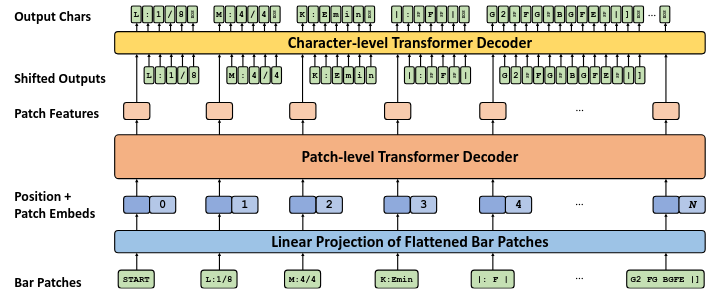
\includegraphics[width=1\textwidth]{IMAGES/NotaGenArchitecture.png} 
\caption{The NotaGen/Tunesformer tokenization and data-processing setup. The patch-level-decoder extracts features for the character level decoder based on which the }
\label{fig:notagenarch}
\end{figure}

\subsection{Control Representation}
We use two different classes of control representation: \textit{discrete labels} and \textit{inner metric or spectral weight profiles}. Both types are derived from the musical onsets of the piece. 
In the lieder dataset the onsets of each voice are projected on to a single musical line, several voices playing at the same time (i.e in chords) are counted as a single onset. The onsets of each piece are arranged on a $96th$ note grid, $24$ notes per quarter note, which allows for integer representation of 16th note triplets and 32nd notes, smaller note values and grace notes (rare in the dataset) are ignored. 
Due to issues discussed in [PUT SECTION REFERENCE HERE], the treatment of onsets in the ragtime dataset varies slightly.
In the ragtime dataset the onsets are taken only from the first voice (in most cases this will be the right hand or a subsection of the right hand) and arranged on a smaller $48$ note grid with $12$ subdivisions per quarter note, smaller note values and grace notes are ignored. 
The comparison of the different control representations is motivated due to their varied granularity and complexity. Note density is captured and controlled for in a variety of ways in several projects on symbolic music generation \cite{Tan_Herremans_2020} \cite{wu2023musemorphose} \cite{Min_Jiang_Xia_Zhao_polyffusion_2023} \cite{Rütte_figaro_2023}, it is simple to evaluate and compare to other models. 
The syncopation labels are the most condensed representation of our target conditioning. 
Inner metric analysis has been successfully used for classification of dance music, detection of meter, study of syncopation. In theory conditi
Spectral weight profiles remain more stable over time but beyond 



\subsubsection{Note Density} For the \textit{discrete label} representation, each bar of the piece is labeled in regard to note density and syncopation levels. For \textit{note density}, all unique onsets across all voices are extracted, the note density is defined as the average distance between two consecutive onsets:
$$
density = \frac{1}{|onsets|}\sum_{n \in onsets}i_j-i_{j-1}
$$
The labels are chosen according to hard coded borders, with 6 classes: $borders = <[3,6,8,12,18,24,48]>$, in a 96 note grid, a label 1 indicates the region 3-6 which is a sixteenth note texture or smaller, while a label 6 indicates the region 24-48, which ranges from a quarter to half-note texture. Averages exceeding 48, or smaller than 3 are clamped to the closest border. \\
\subsubsection{Syncopation Levels}
For \textit{Syncopation Levels} Bemman \cite{Bemman2024} proposes a method to calculate syncopation levels of a sequence by taking the chi-squared distance  between the folded inner metric weight of a sequence  $P_i$ and a meter dependent non-uniform distribution based on beat-strength $S_i$. 
 
We extend the measure to accept a higher resolution grid, with 24 subdivisions per quarter note and verify its performance on the song2014 dataset.  We use following procedure.

\begin{algorithm}\label{algorithm:innermetricweight}
\caption{Calculate Syncopation Score}
\begin{algorithmic}[1]
\Require{Time signature, desired  granularity, Onsets of current bar $B$}
\State Create a nominal distribution $S$ by calculating the beat strength of each beat position at the desired granularity and time signature.\cite{conf/ismir/CuthbertA10}
\State $B_{12}$ = Repeat $B$ twelve times
\State $P_l$ = Extract the inner metric weight profile of $B_{12}$.
\State $P$=Fold $P_l$ into a single bar by summing metric weights at corresponding grid positions across bars.
\State Normalize $P$ and $S$ so that its values fall between 1 and 0
\State 
\[
\text{syncopation score} = 
\sum_{i=0}^{n-1} \left( \frac{(P'_i - S'_i)^2}{P'_i + S'_i} \right)^a
\]
\end{algorithmic}
\end{algorithm}

The parameter $a$ is a weighing parameter and tuned to maximize the correlation of the syncopation score and human ratings of syncopation levels in the song2014 dataset.

Our revised method at higher resolution achives a similar spearman ranked correlation on the song2014 \cite{chunyang2015a} dataset of simple rhythms and perceptual ratings as Bemman with a correlation of 0.624 compared to the reported 0.66 for the measurement using metric weight and nominal weights. 

Since IMA requires at least three evenly spaced onsets to create a local meter, it is generally less effective for short sequences. Therefore, to calculate the syncopation score for a single bar, the bar is first repeated 12 times, then the inner metric weight profile is extracted, folded and normalized as in \ref{algorithm:innermetricweight} 

This process is applied to every bar in the dataset to calculate a per-bar syncopation score per piece. The syncopation labels are calculated by splitting the syncopation scores into 6 quantiles across the entire dataset. 

\subsubsection{Continuous Representation}
We also use the spectral weight profiles (SPW) directly as a conditioning mechanism. 
The profiles are aligned by bar with respect to each bars' meter to accommodate for shifting meters. To balance dataset-compatibility with conditioning size, we limit the meters in the dataset to meters with a ratio of 1.5 (i.e 3/2 is allowed but 4/2 not). The length of the SPW vector is $resolution \times max_ratio = 96 \times 1.5 = 148$. The unused space of the vectors is set to 0.  





\subsection{RhyGen}
We propose RhyGen, a fine-tuned variant of MusicLang with controls for inner metric weight. The fine-tuning targets the \textit{controlled continuation} and the \textit{controlled generation} modes of the model. Here the user provides a MIDI file as input from which inner metric weight is extracted and passed to the model. In \textit{controlled continuation} the user provides two MIDI files, one from which the model continues and one from which the model extracts the target metric weight profile. 

\subsection{Last Minute Gig - extending the game} \label{section:gameext}
Last Minute Gig \cite{Chalkiadakis_2022} is a Musical Attention Control Training game aimed to help people with Parkinson's improve attention control. This is achieved through repeated sessions of play, where a player improvises along to music and is encouraged to change their playing when the music changes. The music is generated using a simple process described below.

\begin{lstlisting}[language=Python]
    # Randomly select initial parameters
    key = random.choice(keys)
    rhythm = random.choice(rhythms)
    chord_progression = random.choice(chords)
    tempo = random.choice(tempos)
    
    pool = ["keys", "rhythms", "chords", "tempos", "is_playing"]
    for bar in range(0,8):
        play_percussion(tempo, rhythm, bar)
        
        if button_pressed():
            play_guitar_chord(chord_progression[bar])
        
        if(bar==7):
            for param in pool: 
                if random.choice([True, False]):
                    change_parameter(param)
            bar = 0 #trigger loop again
    \end{lstlisting}
    
This simplistic generation process has some key limitations, it only changes every 8 bars, which means the music becomes predictable over time, requiring less attention of the participant, potentially reducing the effect of the intervention. The feedback is very limited, the player only a drum loop and the hears guitar chords that they triggered. Finally, all adjustments are random, they cannot take the players current performance in the game into account. Schlette \cite{Schlette_2022} attempts to improve Last Minute Gig, by introducing feedback and dynamically increasing the difficulty of the music. Specifically they replace the pool of possible drum-loops with loops grouped by levels of syncopation. As the player progresses, the drum-loops chosen by the algorithm become more syncopated, resulting in higher difficulty for the player to follow the music. With IMA \ref{section:ima} one can automatically assess syncopation levels in a piece of music, which corresponds to the difficulty of following the music. Our proposed model RhyGen, uses IMA as a control method for music generation to dynamically adjust the perceived difficulty of a generated piece. At the same time the model is capable of multi-instrument generation, which should result in richer more varied music as opposed to the drum and player triggered guitar chords in the original game.

\section{Developing the Model}


\subsection{Preliminary Experiments - proof of concept}
The current methods of adding musical control to an existing model are poorly systematized and rarely compared to each other. While this thesis does not aim to provide a systemic comparison and experimental evaluation of different control methods, some preliminary experiments are necessary to establish an informed course of action. We use BassCraft, a smaller model, and start by controlling for note density. Note density is more easily calculated, tokenized, and verified than inner metric weight. Once control for note density is established, we will move on to inner metric weight. BassCraft is used as a proof of concept for the methods of adding control, it is not part of the final model and evaluation. The most promising approach, or combination of approaches will be applied to fine-tune MusicLang. 

\subsubsection{BassCraft -  a tiny transformer model}
To avoid wasting computing resources and energy, we perform the preliminary experiments on a smaller model: Basscraft. BassCraft is a small transformer model based on GPT2 \cite{Radford_Wu_Child_Luan_gpt2_2019}. It has an embedding size of 256, 4 attention heads, four hidden transformer layers, and 7 million trainable parameters. In contrast, the target LLAMA 2-based model MusicLang has over 100 million trainable parameters. Basscraft generates a bassline to a provided piece of music and is trained on the Lakh MIDI dataset \cite{Raffel_2016}. For training, songs with bass lines are selected (based on the presence of particular MIDI-instrument channels). The tracks are divided into snippets between 1 and 16 bars long. The bass lines are separated from the remaining track and matched as potential output. 
For inference, the user provides a $target$ MIDI file and a MIDI bass instrument such as a Cello, or Electric Bass (see the appendix \ref{midi-bass}) for a full list of MIDI-bass instruments. The $target$ MIDI file can be a single instrument or multi-instrumental track. The model generates a corresponding bass line of the same length as the target file (up to 16 bars). When we add control for note density, the user provides a single integer or a list of integers. If a single integer is passed, that integer is replicated across all generated bars. If a list of integers $X$ of size $|X|$ is provided, then the note density of bar $m$ is given by $X_{m\%|X|} \forall m \in target$.
When control is added for inner metric weight, the user provides an additional reference MIDI file $reference$. The metric weight profile $W$ is given per bar $m$: $W_{m}$. The target rhythmic weight of a bar is given by $W_{m\%|W|} \forall m \in target$. The modulo operation ensures that for note-density and rhythmic weight control, the length of the control input does not have to match the length of the target midi file.    

\begin{figure}[H]
\centering
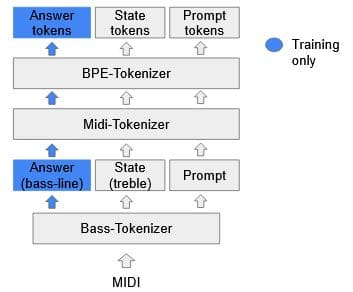
\includegraphics[width=0.5\textwidth]{IMAGES/Preprocessing1.jpg} 
\caption{Preprocessing and tokenization of the original BassCraft model}
\label{fig:preprocessing1}
\end{figure}

\subsubsection{Method 1 - Vocabulary Expansion}

Vocabulary expansion is the process of adding new vocabulary to a transformer model. MusicLang achieves its extraordinary controllability similarly to FIGARO \cite{Rütte_figaro_2023} using control tokens that summarize features of the music that go beyond simply representing MIDI-like events. In vocabulary extension, it is critical to ensure that additional tokens do not overwrite or collide with the existing training. Otherwise, the benefits of using a pre-trained model disappear. Since we use a BPE tokenizer, it is difficult to add new tokens, as it would require retraining the BPE tokenizer, which will transform the embedding layer, making the pre-trained model unusable. Instead, we investigate whether there are unused tokens and reassign them to our new control tokens. These new tokens are not included in any compound tokens generated by the BPE process, which increases the sequence length.

\begin{figure}[H]
\centering
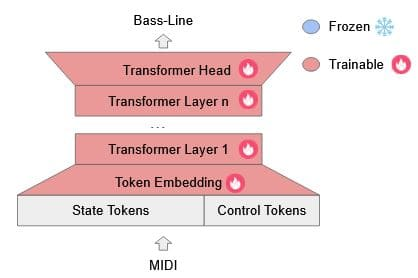
\includegraphics[width=0.5\textwidth]{IMAGES/full_ft.jpg}
\caption{Vocabulary transfer with full fine tuning}
\label{fig:vocabtrans1}
\end{figure}

\begin{figure}[H]
\centering
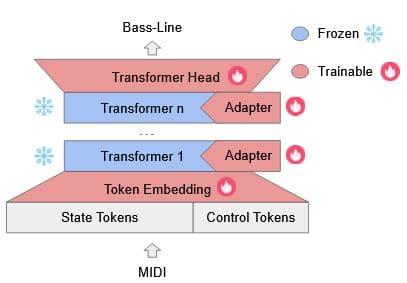
\includegraphics[width=0.5\textwidth]{IMAGES/vocab_lora_ft.jpg} 
\caption{Vocabulary transfer with parameter efficient fine tuning}
\label{fig:vocabtrans2}
\end{figure}

\subsubsection{Method 2 - Integrating of control tokens} 

This approach differs from vocabulary expansion because it processes the control tokens as a parallel to the other input tokens. This is adapted from the approach used in Coco-Mulla \cite{Lin_cocomulla_2024}. After passing through a trainable positional embedding, the parallel stream of control tokens is inserted into the model at a layer $c$. The benefit of this method is that it doesn't require editing the model's vocabulary. 

\begin{figure}[H]
\centering
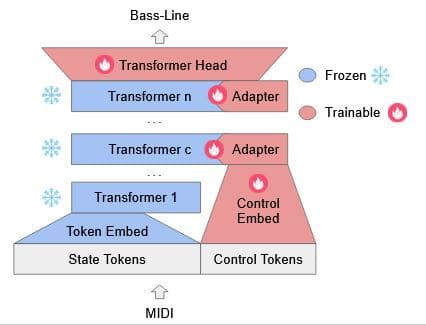
\includegraphics[width=0.5\textwidth]{IMAGES/ControlTokensLora.jpg} 
\caption{Integration of control tokens with parameter efficient fine tuning}
\label{fig:controltok}
\end{figure}

\subsubsection{Method 3 - Post-Hoc Guidance and other improvements}

SMITIN\cite{Koo_Wichern_Germain_SMITIN_2024} uses post-hoc guidance on a trained model to influence the generation process without retraining the model. This type of sampling-based guidance has been very successful in diffusion models. In transformers for sequence generation, however, it produces mixed results \cite{language_guide_rutte_2024}. Additionally, this may be difficult to implement and transfer to IMA. Both SMITIN and Rütte \cite{language_guide_rutte_2024} only use one-dimensional variables that indicate the probability of a concept being present or not. Both note-density and IMA are non-binary features, which complicates the mapping of this guidance strategy to our proposed model. 

\begin{figure}[H]
\centering
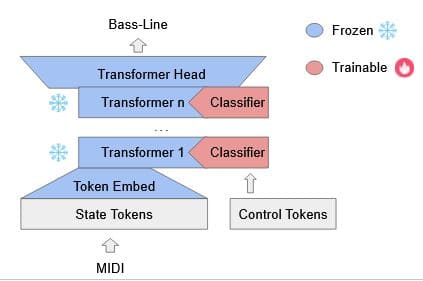
\includegraphics[width=0.5\textwidth]{IMAGES/adhoccontrol.jpg} 
\caption{Integration of control using inference time interference}
\label{fig:adhoccontrol}
\end{figure}

If these experiments are unsuccessful, we can follow the approach of \cite{Shu_Xu_Musebarcontrol_2024} and try additional training using auxiliary tasks or a modified (counterfactual) loss function. 

\subsection{Using inner metric weight as controllable feature}
Inner metric analysis (IMA) creates metric weight profiles we use as guiding features passed to the model bar by bar, which allows us to induce shifts in metric weight in the output. 
For this, we use the globally smallest available note grid of the Lakh MIDI dataset $g_{min}$. The calculated rhythmic profile is normalized and provided to the model as a vector of length $g_{min}$. 
The model then learns embeddings of the distribution alongside positional embeddings \cite{Lin_cocomulla_2024}. These embeddings are incorporated into the model. 
The model is trained by providing a piece as a MIDI file, this is then split into two streams. On the one hand, the MIDI file is tokenized, on the other hand, the rhythmic profile is extracted from the MIDI file. The model is trained on both the embeddings of the extracted profile and the tokenized MIDI file. 
For inference, the user can provide a reference track from which the inner metric profile is extracted and passed to the model. 

\subsection{Training RhyGen}
Methods 1, 2, and 3 are sorted by expected difficulty of implementation. We first implement these methods on BassCraft since the model is only a fraction of the size of RhyGen and therefore easier to train and iterate on. First, BassCraft is extended using each method with control for note density. When a method is found that introduces sufficient control, we extend this to IMA and try generating basslines with a provided metric profile. Finally, the most promising method (or combination of methods) is adopted to MusicLang, creating RhyGen.


\section{Model Evaluation}
\subsection{Custom Datasets}
The following table describes the datasets we will construct, their purpose, and their breakdown. 
\begin{table}[H]
    \centering
    \renewcommand{\arraystretch}{1.3}
    \begin{tabular}{|l|p{4cm}|p{7cm}|}
        \hline
        \textbf{Name} & \textbf{Aspect} & \textbf{Description} \\
        \hline
        \texttt{lmd1000} & Fine-tuning Dataset & 1000 songs from Lakh MIDI Dataset \cite{Raffel_2016} (containing bass-lines so we can use it to train both RhyGen and BassCraft) \\
        \hline
        \texttt{lmd500} & Evaluation Dataset & Randomly selected subsection of 4 to 16 bars of 500 songs not in \textit{lmd1000} \\
        \hline
        \texttt{srhythm} & Evaluation of rhythm control & 30 manually chosen prototypical rhythms based on \cite{Chew_Volk_Lee_Dance_metric_weight_2005} Tango, Rumba, Bossa Nova, Merengue, and March \\
        \hline
        \texttt{schord} & Evaluation of chord control & 30 two-, three-, and four-bar chord progressions \\
        \hline
        \texttt{bcraft\_inf} & Preliminary BassCraft Evaluation & BassCraft applied to \texttt{lmd500} with randomly chosen rhythms from \texttt{srhythm}, this is used for development purposes \\
        \hline
        \texttt{mlang\_inf\_con} & RhyGen Controlled Generation & RhyGen applied to 500 chord-rhythm pairs from \texttt{schord} and \texttt{srhythm} \\
        \hline
        \texttt{mlang\_inf} & RhyGen Controlled Continuation & RhyGen applied to \texttt{lmd500}, continuing excerpts with randomly chosen rhythms from \texttt{srhythm} \\
        \hline
    \end{tabular}
    \caption{Summary of datasets used for fine-tuning and evaluation}
    \label{tab:dataset_summary}
\end{table}


%For fine-tuning the models with new control mechanisms, we use a small random subset of 1000 songs from the Lakh MIDI Dataset $lmd1000$. For BassCraft, we ensure that all songs in $lmd1000$ contain bass lines. Both BassCraft and RhyGen are evaluated objectively using a second random subset of 500 songs from which a random subsection between 4 and 16 bars is selected for the \textit{continuation} mode of RhyGen and the bass generation of BassCraft. This is the $lmd500$ evaluation dataset. The references for inner metric weight come from a small set of $n=30$ manually chosen prototypical rhythms $srhythm$ using the set by \cite{Chew_Volk_Lee_Dance_metric_weight_2005} of prototypical rhythms for Tango, Rumba BossaNova, Merengue, and March as a starting point. This can be expanded as desired for showcasing the control effectiveness.
%To evaluate combined control of chords and rhythm we create a small set $n=30$ of different two, three, and four-bar chord progressions.
%Finally, we create three datasets containing inferences from the model for evaluation, $bcraft\_inf$,  $mlang\_inf\_con$, $srhythm$. Each contains 500 entries, the model weights remain frozen during this process.  
%To evaluate BassCraft we create $bcraft\_inf$ by running BassCraft on $lmd500$ with a randomly chosen rhythm from $srhythm$ as a control condition for each section in $lmd500$. 
%To evaluate RhyGens's \textit{controlled generation} mode we create $mlang\_inf\_con$ by running RhyGen on 500 different pairwise permutations of chords from $schord$ and rhythms from $srhythm$. 
%To evaluate RhyGen's \textit{controlled continuation} we run RhyGen on $lmd500$ with randomly chosen rhythms from $srhythm$ for each track to create $mlang\_inf$, where RhyGen continues from the excerpt from $lmd500$.  

\subsection{Evaluating Control-Effectiveness}
As discussed in section \ref{section:evaluation}, calculating whether or not the control is effective depends on the controlled feature but can happen automatically. 
The first set of experiments targets note density: 
%If note density is a categorical variable such as low, medium, or high, the error is calculated similarly to a multilabel classifier. The predicted label is the note density of the generated music, and the ground-truth label is the note density given in the prompt on a bar-by-bar level. 
%The metrics include accuracy, precision, recall, and F1 scores. 
Note density is continuous (the number of notes per bar), so we can calculate the error between the desired note density and the generated note density as the mean square error: 
\begin{equation}
 error_{continuous} = \sqrt{\frac{1}{n}\sum_{j=1}^{n}(y_{generated}-y_{prompt})}
\end{equation}
Inner metric weight analysis generates metric weight profiles, which we use as a guidance mechanism. Following the approach by \cite{Bemman2024}, we can compare the generated and the target rhythmic weight profiles using chi-squared distance.
Given target distribution $T$ and generated distribution $G$, the distance is given by 
\begin{equation}
D=\sum_{i=0}^{n-1}(\frac{(T_i-G_i)^2}{T_i+G_i})
\end{equation}
The target distribution is the rhythmic template, and the generated distribution is the generated output conditioned with that rhythmic template. A smaller difference indicates better control effectiveness. 

\section{User Study}
\textbf{RQ2} and \textbf{RQ3} are evaluated through a user study. The goal is to recruit $n=20$ participants to complete a test of interactability and a survey comparatively evaluating the generated music. 
\subsection{Interactive Study}
The interactive study aims to evaluate the fitness of the controlled generated music from an MACT perspective. Specifically, in the MACT protocol used by Chalkiadakis \cite{Chalkiadakis_2022}, the patient is supposed to listen to changes in the music and change their playing. There are two options that we are deciding between, both options will operate on $n=5$ pieces that are generated using RhyGen in the \textit{controlled generation} condition, with rhythm controls at several points in the piece. For this, we provide the model with a MIDI file consisting of rhythm changing at 8-bar intervals concatenated into one file.
For comparison with the previous system, we generate an additional $n=5$ pieces using the approach by Chalkiadakis \cite{Chalkiadakis_2022} with the algorithm described in section ref{section:gameext}. To reduce potential confounds the RhyGen generation will follow Chalkiadakis's constraint of initiating changes every 8 bars, though the system is more flexible than that. Chalkiadakis algorithm will be restricted to changes in rhythm, though it is capable of other changes.\\\\
\textbf{Option 1}
In our simplified interactive sessions, we ask the player to hit a button whenever they hear a change in the music. The button presses are registered alongside the starting time, tempo, and registered changing points (determined from the prompt). Finally, we correlate the timing of the button presses and registered changes are correlated with each other. A high correlation indicates that the participants noticed the changes. 
\textbf{Option2}: We ask players to tap along to the music, and change their tapping when they notice a change. We analyze the regularity of the taps matching them with the music playing and investigate them for changes. 

\textbf{Hypothetical hypotheses}: 
\begin{itemize}
\item \textbf{P1} There is no difference in the abilities of recognizing changes between the systems.
\item \textbf{P2} Players have more difficulty recognizing changes between certain rhythmic changes than others.
\item \textbf{P3} Players have more difficulty following music generated with certain rhythmic templates than others.     
\end{itemize}

For P1 (in option 1) we calculate recognition accuracy by comparing the timing of the button hit, with the timing of the change. $recognition\_accuracy = |t_{hit}-t_{true}|$. Then we test the difference of average recognition accuracy between groups for significance using a t-test with $\alpha=0.05$. In option 2 this is more complex. We would measure the distances between the player taps. The point in which we detect the largest change in average tap distance is $t_{rec}$. Rocognition accuracy is calculates as $recognition\_accuracy = |t_{hit}-t_{true}|$, then we perform the t-test as described above. 
For P2 we take recognition accuracy as calculated above, and group them by the five different rhythmic conditions we created. Each of the five rhythmic conditions is then compared with each other using repeated t-tests with $\alpha=0.05$\\  
P3 is only relevant in option 2. Here the users tapping is quantized to the smallest rhythmic value of the reference rhythm. The rhythmic profile of the user's tapping is extracted using IMA, and then the chi-squared distance between the rhythmic profile of the tapping and the rhythmic profile of the music is calculated. This is calculated for each of the five rhythmic conditions, and then compared as above using repeated pairwise t-tests with $\alpha=0.05$

\subsection{Survey}
The survey will compare the listening experience of our model to the rule-based music generation system used in the original game to answer RQ3, whether the music by RhyGen improves listener experience.  The survey will also include the original MusicLang, to assess whether or not the fine-tuning for rhythm control decreases other capabilities of the model. Optionally, we include other symbolic music generators such as FIGARO \cite{Rütte_figaro_2023}, this will help provide a point of comparison. Following the recommendation of \cite{Yin_Reuben_Stepney_Collins_2023} we could also include a state-of-the-art rule-based generator such as MayaMarkov \cite{Collins_Laney_2017} and human-composed music from the Lakh MIDI dataset. 
The questionnaire will be adopted from \cite{Yin_Reuben_Stepney_Collins_2023}, and each musical excerpt will be rated on a 7-point Likert scale along the following dimensions: aesthetic pleasure, repetition, melody, harmony, and rhythm.\footnote{From \cite{Yin_Reuben_Stepney_Collins_2023}: Aesthetic pleasure (Ap) The extent to which someone finds beauty in something 
Repetition or self-reference (Re) The reuse, in exact or inexact form, of musical material (e.g., notes, melody, harmony, rhythm) within a piece.
Melody (Me) A succession of notes, varying in pitch, which have an organized and recognizable shape. Melody is horizontal, i.e. the notes are heard consecutively.
Harmony (Ha) The simultaneous sounding of two or more notes; synonymous with chords. The organization and arrangement of chords and their relationships
to one another, vertically (at the same time) and horizontally (across time) throughout a piece
Rhythm: Everything about the time aspect of music (as distinct from the aspect of pitch), including event or note beginnings and endings, beats, accents, measures, and groupings of various kinds.} 
Optionally there is space for the participant to comment on each excerpt. The participant will not see the source of the excerpt (i.e. which model or whether it is generated). 
The music provided for comparison will be excerpts cropped to about 30 seconds of rendered MIDI. While we don't cherry-pick the tracks, we will follow \cite{Yin_Reuben_Stepney_Collins_2023} and filter the music to prevent 1) excessive repetition of a small sequence (the model getting "stuck"), 2) long stretches of silence, 3) verbatim copying of training data or the prompt. 
The questionnaire also includes questions on demographic information such as gender, age, educational background, and musical experience.

\textbf{Hypothetical hypotheses}: 
\begin{itemize}
\item{P1} Ratings of aesthetic pleasure are higher for RhyGen than for Chalkiadakis's rule-based system.
\item{P2} Ratings of aesthetic pleasure are not higher for MusicLang than for RhyGen. 
\item{P3} Ratings of repetition, melody, harmony, and rhythm are positively correlated with ratings for aesthetic pleasure.
\item{P4} Ratings of rhythmic success are higher in RhyGen with certain rhythm conditions than others.
\end{itemize}

For P1 and P2, the average ratings of the groups are compared and tested for significance using t-tests with $\alpha=0.05$. 
For P3 we perform a Pearson-correlation test between each of the musical ratings and ratings for aesthetic pleasure.
For P4 we group the ratings of rhythmic success by rhythm condition and then perform pairwise t-tests with $\alpha=0.05$ for each possible pair of rhythm conditions. 


\subsection{Additional points of discussion}
Beyond simple statistical evaluation, we would include listening examples and an interactive code space on Google Collab where the reader can interact with RhyGen. Additionally, discussing participants' comments, and investigating the model output musicologically could be worthwhile depending on the results. 
\section{Thesis Timeline}

\begin{figure}[H]
    \centering
    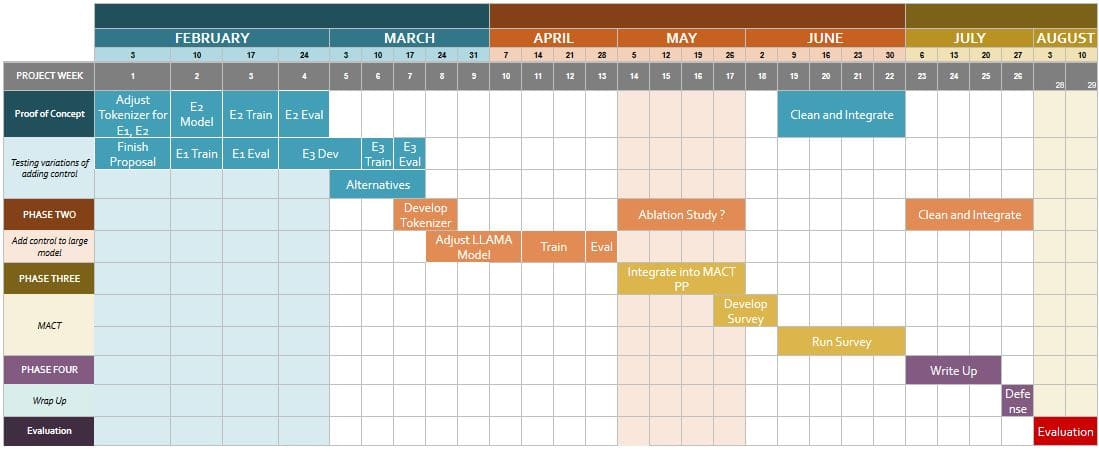
\includegraphics[width=1\textwidth]{IMAGES/project_plan.jpg} 
    \caption{Thesis project plan}
    \label{fig:projectplan}
\end{figure}


